\documentclass[11pt,letterpaper]{article}

\usepackage{fancyhdr}
\usepackage[latin1]{inputenc}
\usepackage{amsmath}
\usepackage{amsfonts}
\usepackage{amssymb}
\usepackage{graphicx}
\usepackage[hmargin=2cm,vmargin=2.5cm]{geometry}
\usepackage[normalem]{ulem}
\usepackage{enumerate}
\usepackage{hyperref}
\usepackage{palatino}

\newcommand{\workingDate}{\textsc{October 2018}}
\newcommand{\courseName}{MTH 201}
\newcommand{\institution}{Grand Valley State University}

\pagestyle{fancy}
\setlength\parindent{0in}
\setlength\parskip{0.1in}
\setlength\headheight{15pt}

%%%%%%%%%%% HEADER / FOOTER %%%%%%%%%%%
\rhead{\workingDate}
\chead{\textsc{Lab 5}}
\lhead{\textsc{\courseName}}

\begin{document}

\begin{flushright}
	\begin{Large}
		Lab 5: Models of infant growth
	\end{Large}
\end{flushright}

\noindent
\textbf{Overview:} Logarithmic functions are important for a host of reasons in real life applications, one of which is that they model data that have a particular shape. In this lab, you'll explore data that have a logarithmic shape, build a computer model for the data, and then use calculus to analyze the growth rates of the model using our newly-formulated derivative rules for logarithmic functions. 

\vskip

\textbf{Technology skills needed for this lab:} Entering data as a table into Desmos and entering a function into Desmos. Please see the instructions for Lab 1 for how to enter data. 



\subsection*{Setup and Instructions}

On the course website where the Lab is posted, you will find an image file that contains a chart from the US Center for Disease Control. The chart shows the growth curves for length (height) and weight of boys born in the US, from birth to age 36 months. This is one chart that contains two groups of curves, and in each group there are seven individual curves. Here is how to read these graphs: 

\begin{itemize}
	\item The upper set of curves describes the length (height) of boys as they grow. The lower set of curves describes weight. 
	\item Within each set, there are seven curves depending on \emph{percentile}. For example, the lowest curve in each set shows the progression of boys who are in the 5th percentile -- that is, boys for whom 95\% of the population are heavier or longer than they are. The curve in the middle shows the progression of boys who are in the 50th percentile -- boys who are in the exact middle of the population in terms of weight or length. 
	\item Finally, note that along the bottom of the chart is a time scale, in months starting from birth up to 36 months. along the left and right sides are weight in pounds and kilograms, and length in inches and centimeters. 
\end{itemize}

The bulk of this lab depends on two graphs you're going to construct based on the CDC data. Follow these directions to set that plot up: 

\begin{enumerate}
	\item Decide whether you would like to study weight, or whether you'd like to study length. Pick one. 
	\item For the critierion you chose (length or weight), find the curve that represents the 50th percentile. 
	\item Open up Desmos and create a new table. 
	\item In the first column of the table, enter time in months, in increments of three months, starting with birth (0 months) and ending at 3 years of age (36 months). So you should end up with 13 entries. 
	\item In the second column, enter in the value of the criterion you chose (length or weight) at each month value (0, 3, 6, .., 36 months). \textbf{You will need to estimate these off of the CDC charts.} Use the image of the charts to zoom in on the charts to get an accurate reading. You may choose either unit of measurement, but make a note of which one you choose. 
	\item You will now have two columns of data: One for age (let's call that $t$, in months) and another for length or height (let's call that $y$). Once you've entered in the data, the data points will appear on the graph. You will probably need to change the window parameters to see all the points --- if you don't know how to do this, read this tutorial: \url{http://bit.ly/2QObIg2}
	\item Back in Desmos, add a new formula below the table and type: 
	\begin{verbatim}
	    y = a * ln(b*x) + c
	\end{verbatim}
	You will be prompted to add sliders for $a$, $b$, $c$, and ``All''. Select ``all''. This creates an interactive graph with three sliders to control the values of $a$, $b$, and $c$. For example, here's the graph of $y = 2.2 \ln(0.6x) - 1.8$: 
	\begin{center}
	    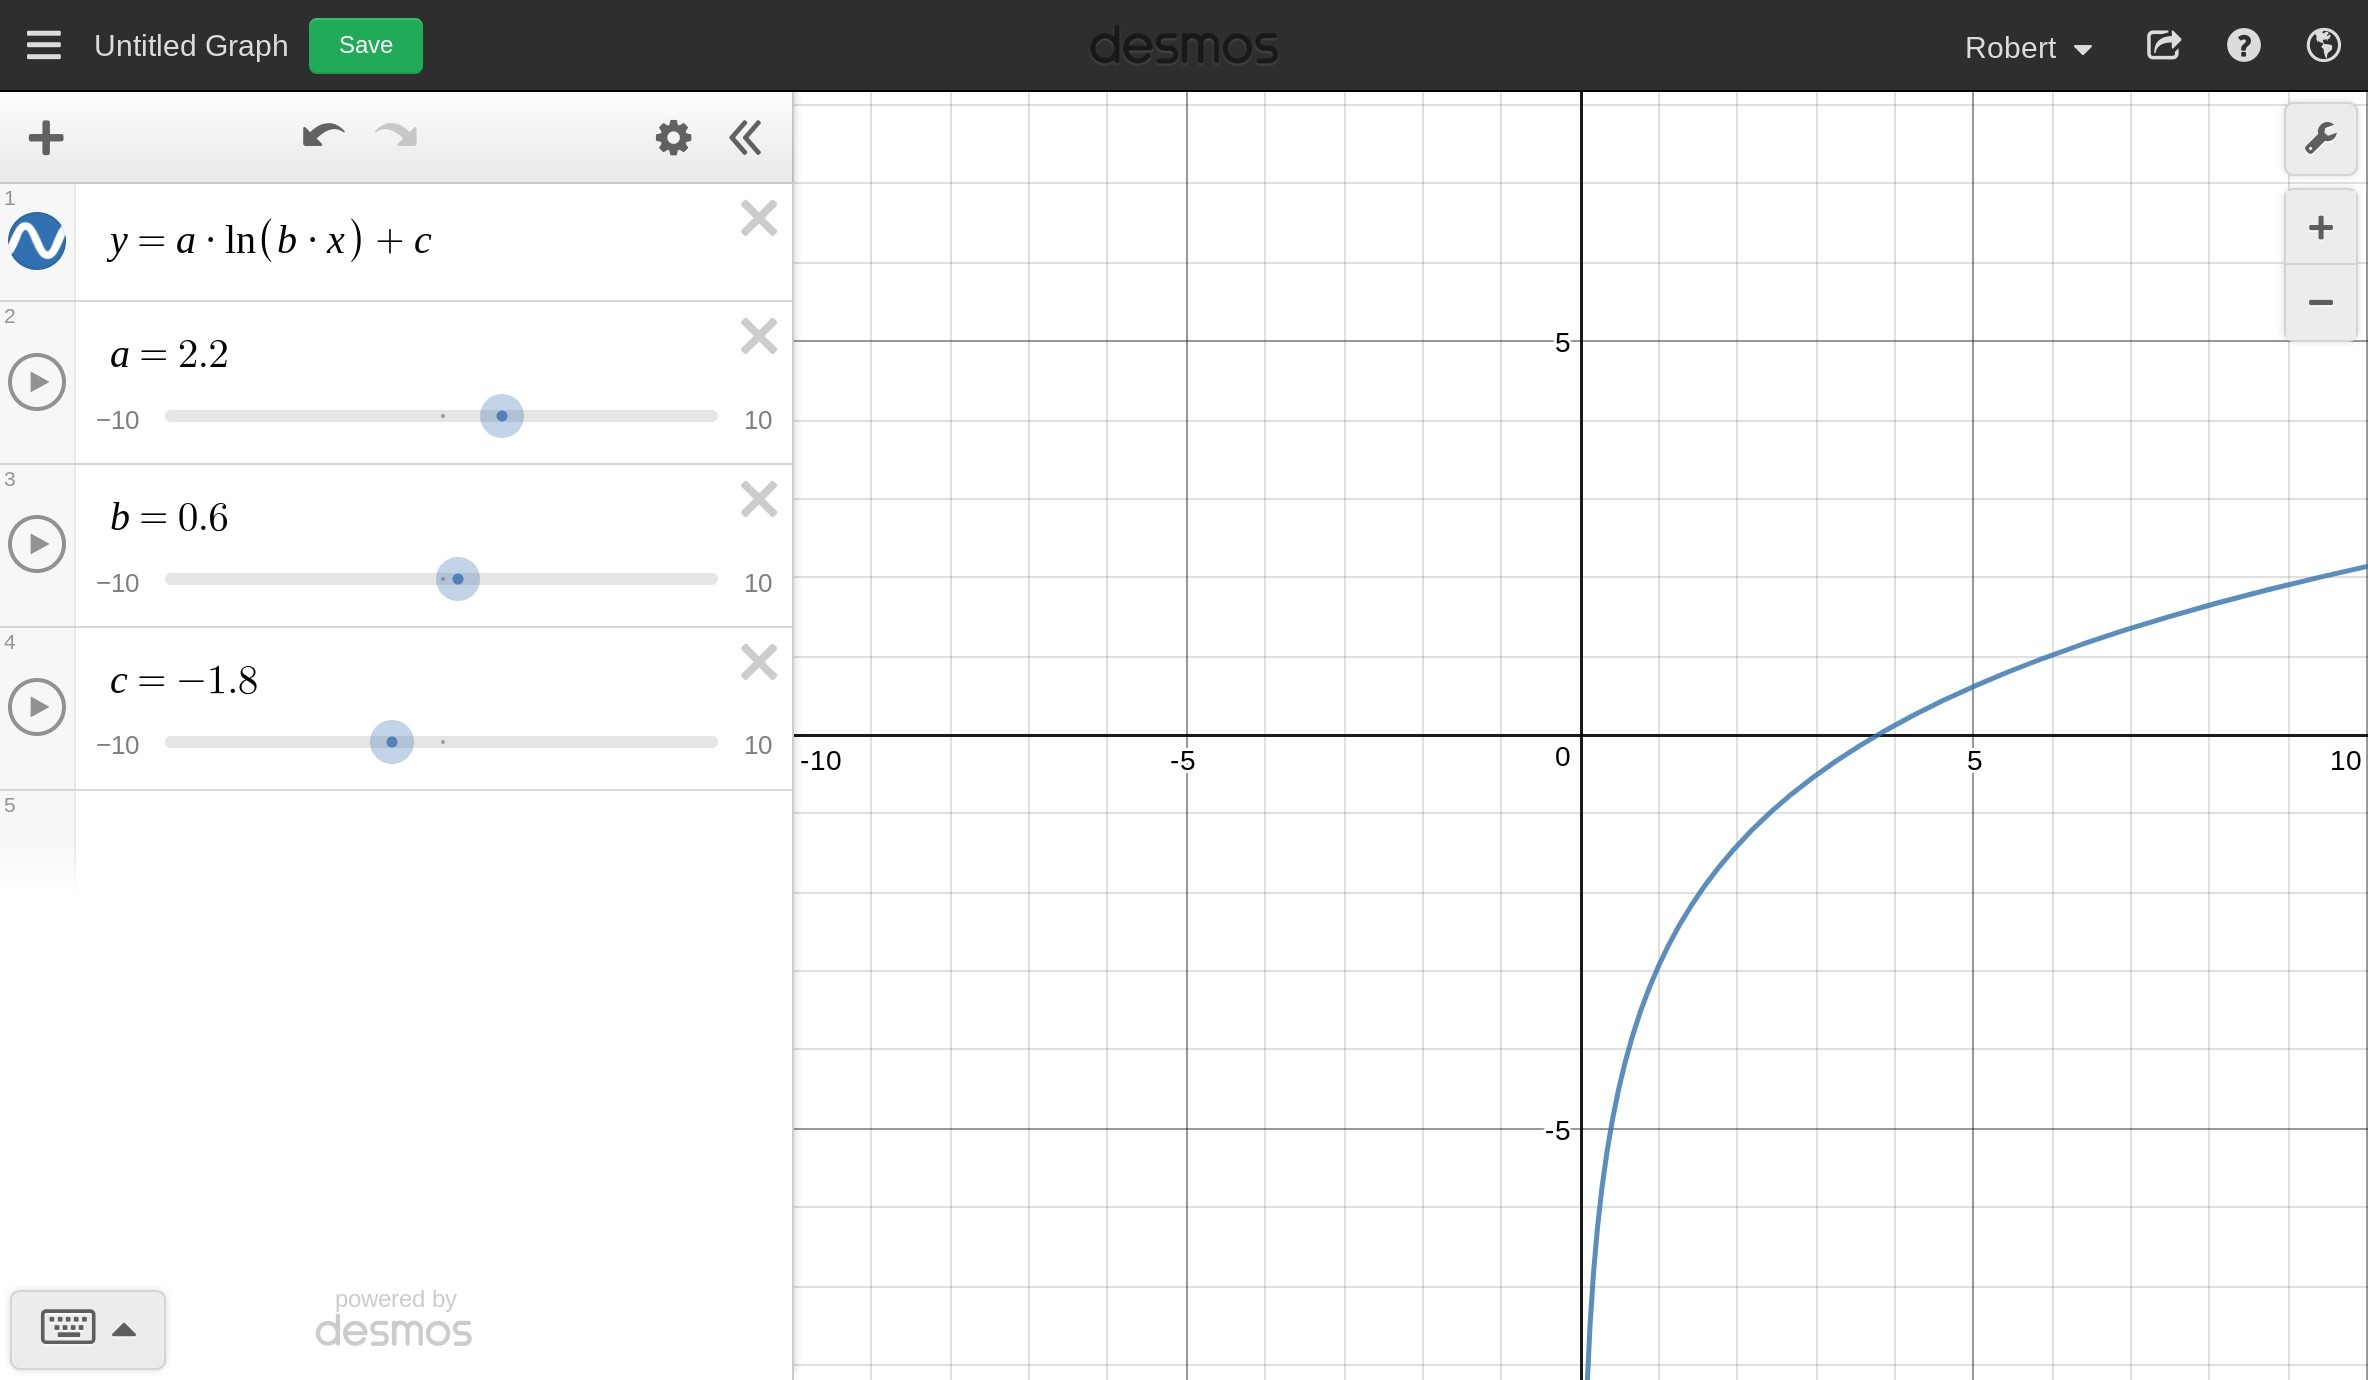
\includegraphics[width=4in]{desmos-lab5.jpg}
	\end{center}
	A video of the entire process of creating this graph is found here: \url{https://drive.google.com/file/d/1JhcDw1hpidSHKPDX8SVT9OBymukEs9X2/view}
	\item As a last step in constructing this interactive graph for the lab, change the top limit on each of the sliders from 10 to 100. To do this, just click on the ``10'' on each of the sliders and change each one to ``100''. 
\end{enumerate}

Keep this window open during your Lab, since you are going to be exploring several different models for the child growth data. 


\subsection*{Main Activities}

\begin{enumerate}
    \item If you followed the setup instructions above, you should have a Desmos graph with two items on it: The 13 data points you estimated off the CDC tables, and a graph. Manipulate the sliders until you have a graph that roughly fits the data. You will probably not be able to obtain a perfect fit, but your graph should stay relatively close to the data and pass through the main arc that the scatter plot traces out. Please note, if your curve is a significantly poor fit, you will probably have to revise this lab. Here's an example of a bad fit: 
    	\begin{center}
	    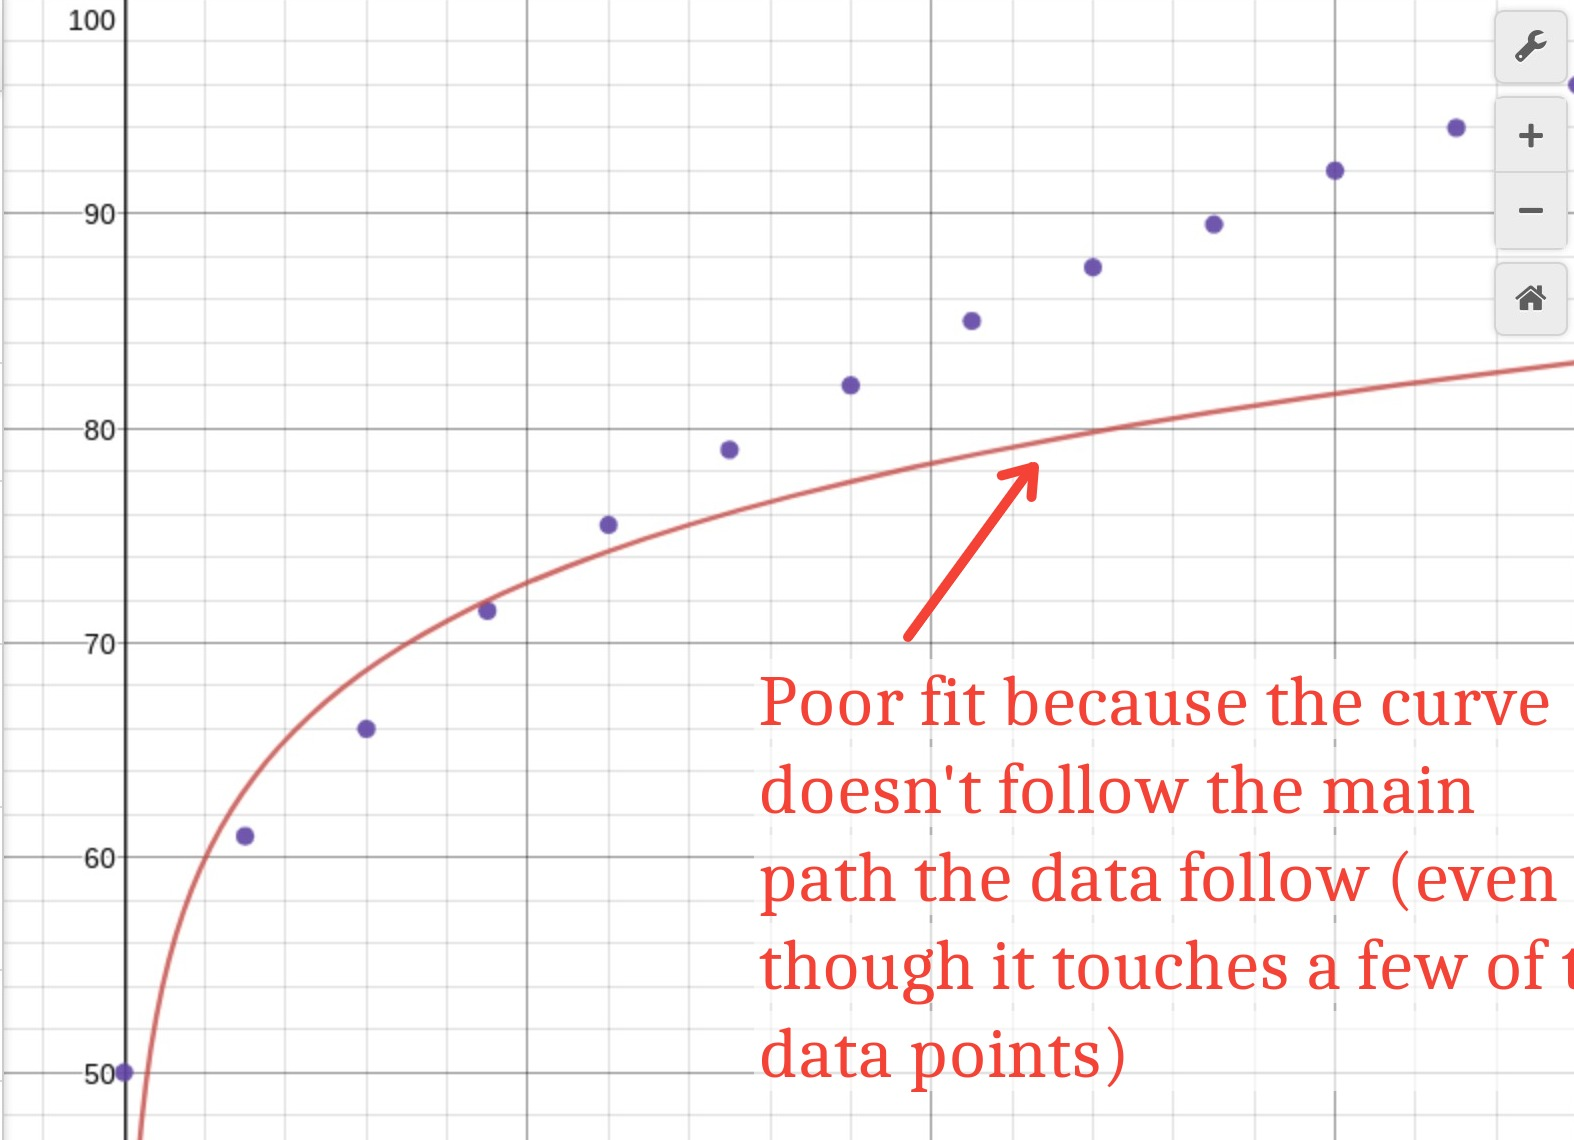
\includegraphics[width=3in]{desmos-lab5-2.jpg}
	\end{center}
	Once you have a good fit, give the link to your Desmos plot in the writeup. 
	
	Side note: This method of fitting a curve to data by hand is called \emph{parameter estimation}. It's an important data analysis technique when regression analysis, like you did in Lab 1, has issues (which it does here because we are using a log function). 
	
	\item Write down the formula for your curve, with the parameter values $a$, $b$ and $c$ filled in. For example, if you found that the best fit was when $a = 5$, $b=2$, and $c=3$, write down $y = 5 \ln (2x) + 3$. 
	
	\item Calculate the first and second derivatives of your model and show your work in the writeup. Then, based on the outcome of the derivatives, discuss the increasing/decreasing behavior of that model and the concavity of that model. (Will the model ever decrease? Will the model ever go completely horizontal? Will the model always have the same concavity, or will the concavity change at some point?) 

	\item Now pretend you are a pediatrician who is working with a new parent (who does not know anything about calculus), who is concerned that their child, being in the 50th percentile, is going to have health issues later on. Translate the technical information about the growth and concavity of your model from the previous question, into a 3-4 sentence paragraph appropriately phrased so that the new parent can understand how their child will grow over the next three years. (Please note, you need to get into character for this part. Explanations that are overly technical or not useful for an ordinary person will have to be redone. Maybe read this off to your roommate or a friend before submitting it.) 

    \item Finally, think about the fact that we used a log function as the base model for this problem. What aspects of the shape of a logarithmic function made this a good choice for a model, as opposed to a linear, power, or exponential model like you've used in the past? In general, if we are choosing types of functions to use to model data, when would we want to start with a log function? 

\end{enumerate}

	
\end{document}